%!TEX root = ../StrinJet.tex

\section{Simulate with PYTHIA 8 rope}%
\label{sec:rope}
\textbf{Parameters}

Beams:idA = 2212
\\Beams:idB = 2212
\\Main:numberOfEvents = 1001
\\Beams:eCM = 13000.
\\SoftQCD:all = on
\\
\\MultiPartonInteractions:pT0Ref = 2.15
\\BeamRemnants:remnantMode = 1
\\BeamRemnants:saturation = 5
\\ColourReconnection:reconnect = on
\\ColourReconnection:mode = 1
\\ColourReconnection:allowDoubleJunRem = off
\\ColourReconnection:m0 = 0.3
\\ColourReconnection:allowJunctions = on
\\ColourReconnection:junctionCorrection = 1.2
\\ColourReconnection:timeDilationMode = 2
\\ColourReconnection:timeDilationPar = 0.18
\\
\\Ropewalk:RopeHadronization = on
\\Ropewalk:doShoving = on
\\Ropewalk:tInit = 1.5 %# Propagation time
\\Ropewalk:deltat = 0.05
\\Ropewalk:tShove = 0.1
\\Ropewalk:gAmplitude = 0. %# Set shoving strength to 0 explicitly
\\
\\Ropewalk:doFlavour = on
\\Ropewalk:r0 = 0.5
\\Ropewalk:m0 = 0.2
\\Ropewalk:beta = 0.1
\\
\\!// Enabling setting of vertex information.
\\PartonVertex:setVertex = on
\\PartonVertex:protonRadius = 0.7
\\PartonVertex:emissionWidth = 0.1

\begin{figure}[ht]
	\begin{center}
		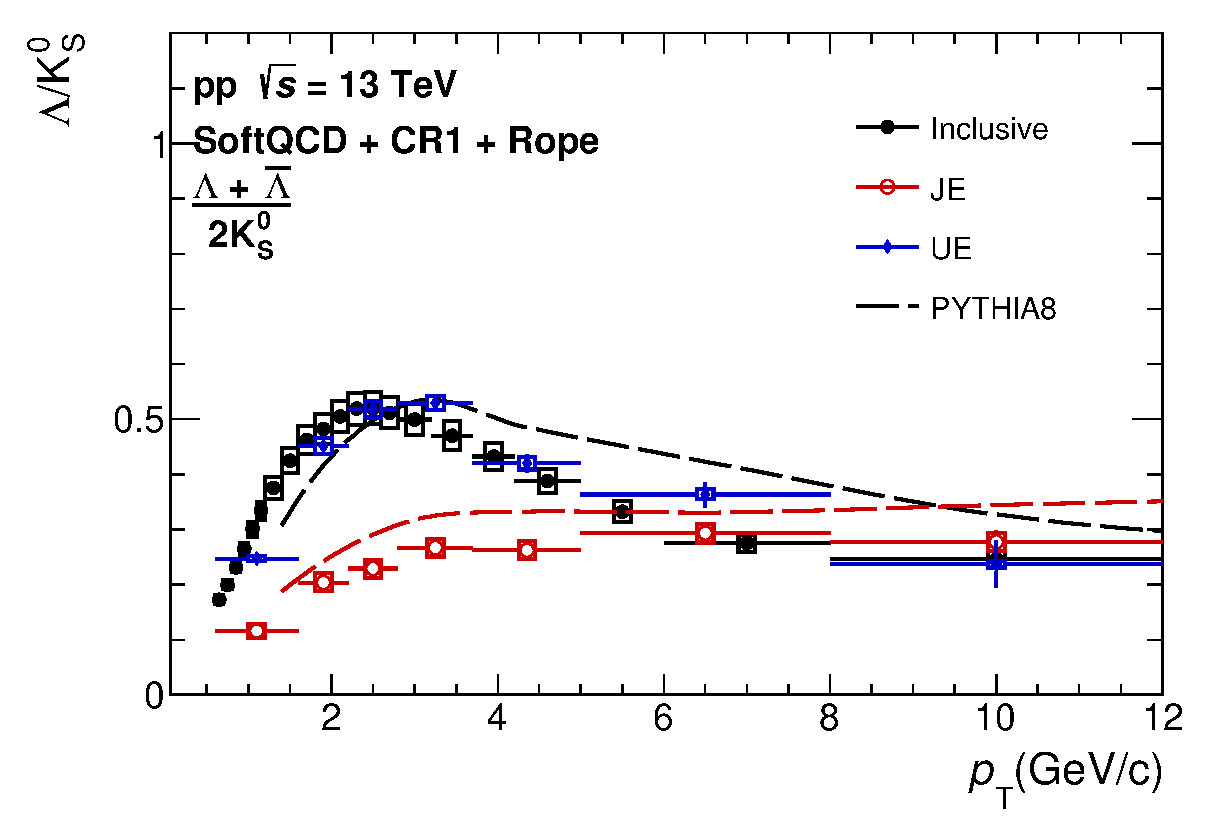
\includegraphics[width=.3\textwidth]{Lambda_sum_toKRatio_DataPy_Rope_sQCD}
		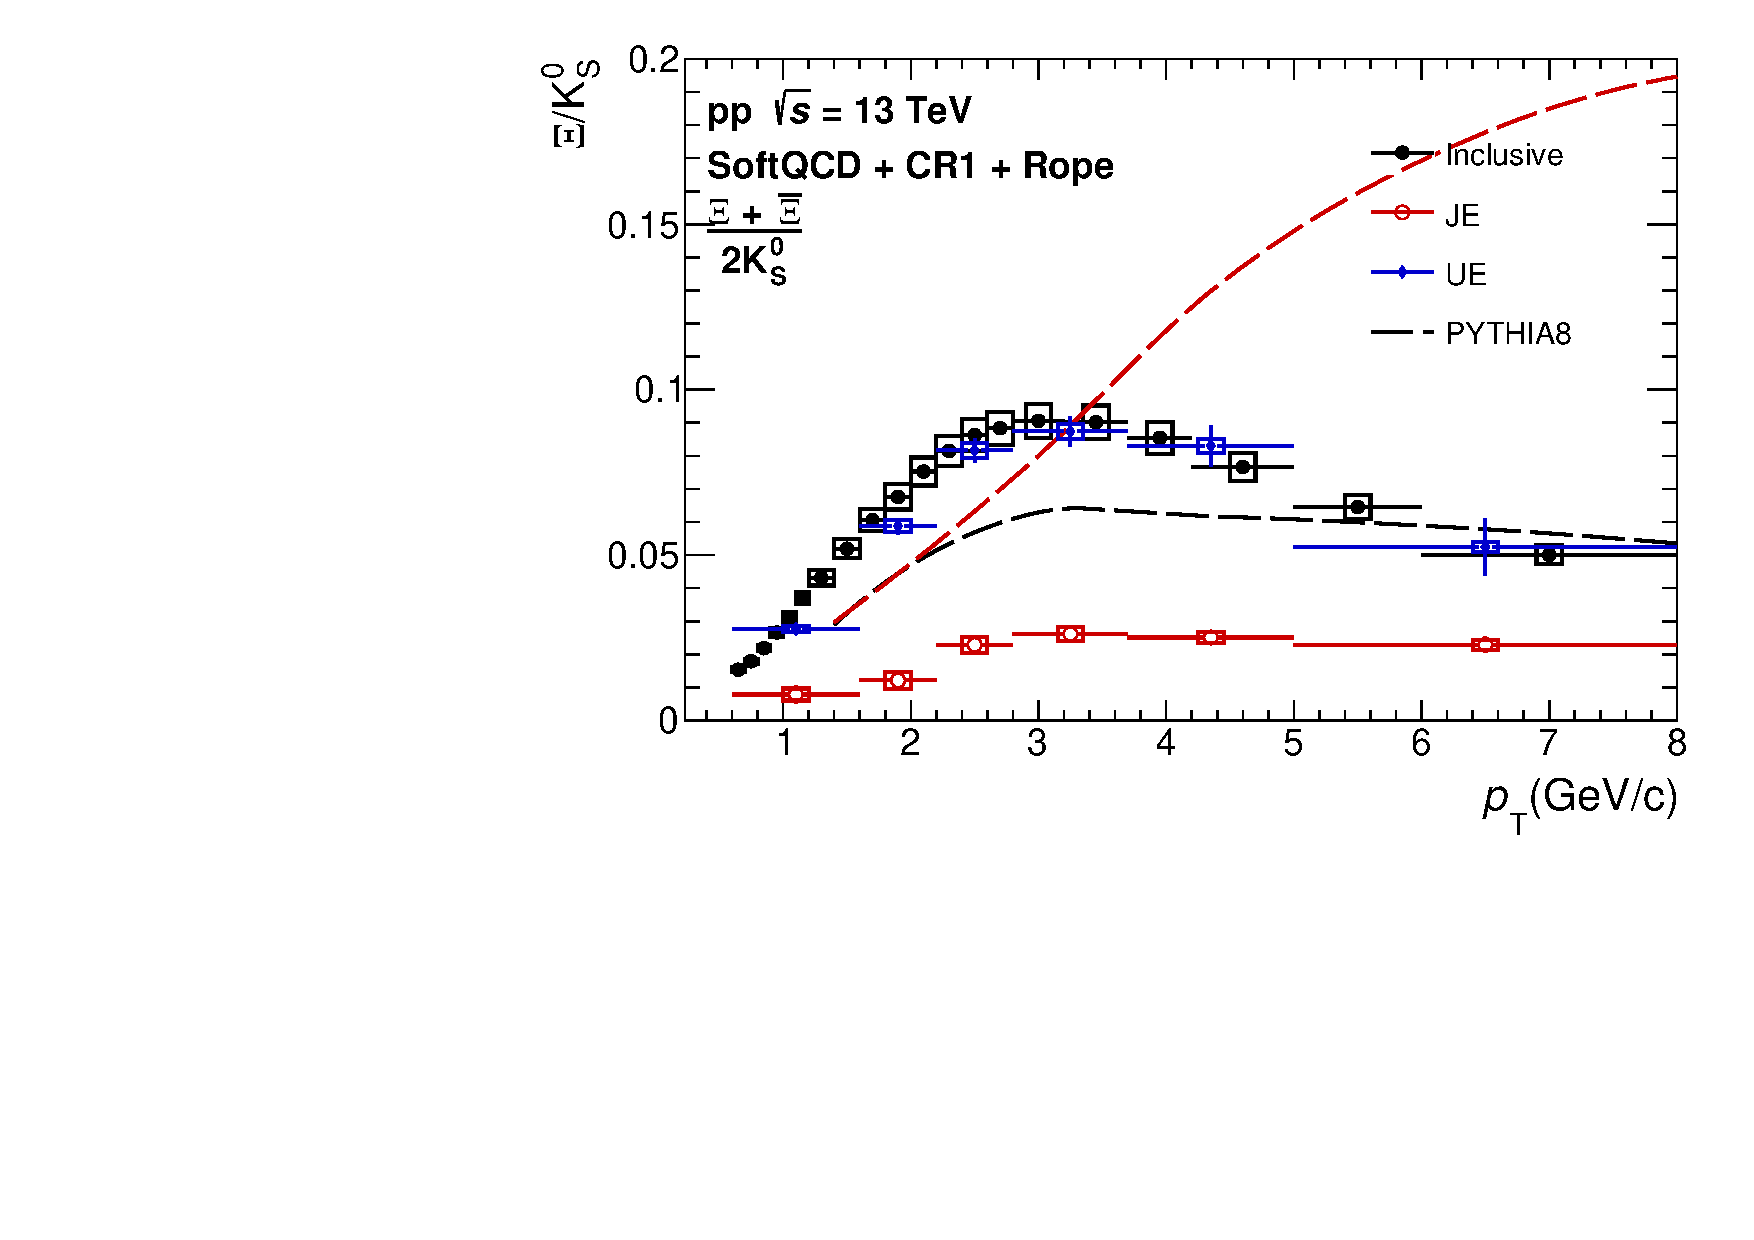
\includegraphics[width=.3\textwidth]{Xi_toKRatio_DataPy_Rope_sQCD}
		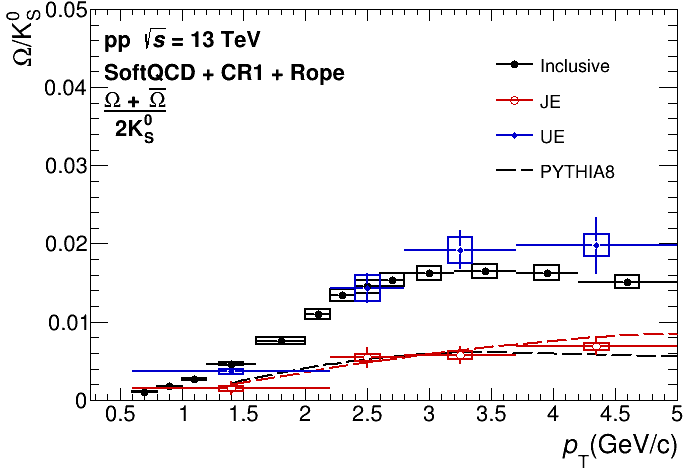
\includegraphics[width=.3\textwidth]{Omega_toKRatio_DataPy_Rope_sQCD}
	\end{center}
	\caption{.}
	\label{fig:SMParticle}
\end{figure}
